\chapter{Preface}

\section*{Pulse sequence notation}

\begin{figure}[ht]
    \centering
    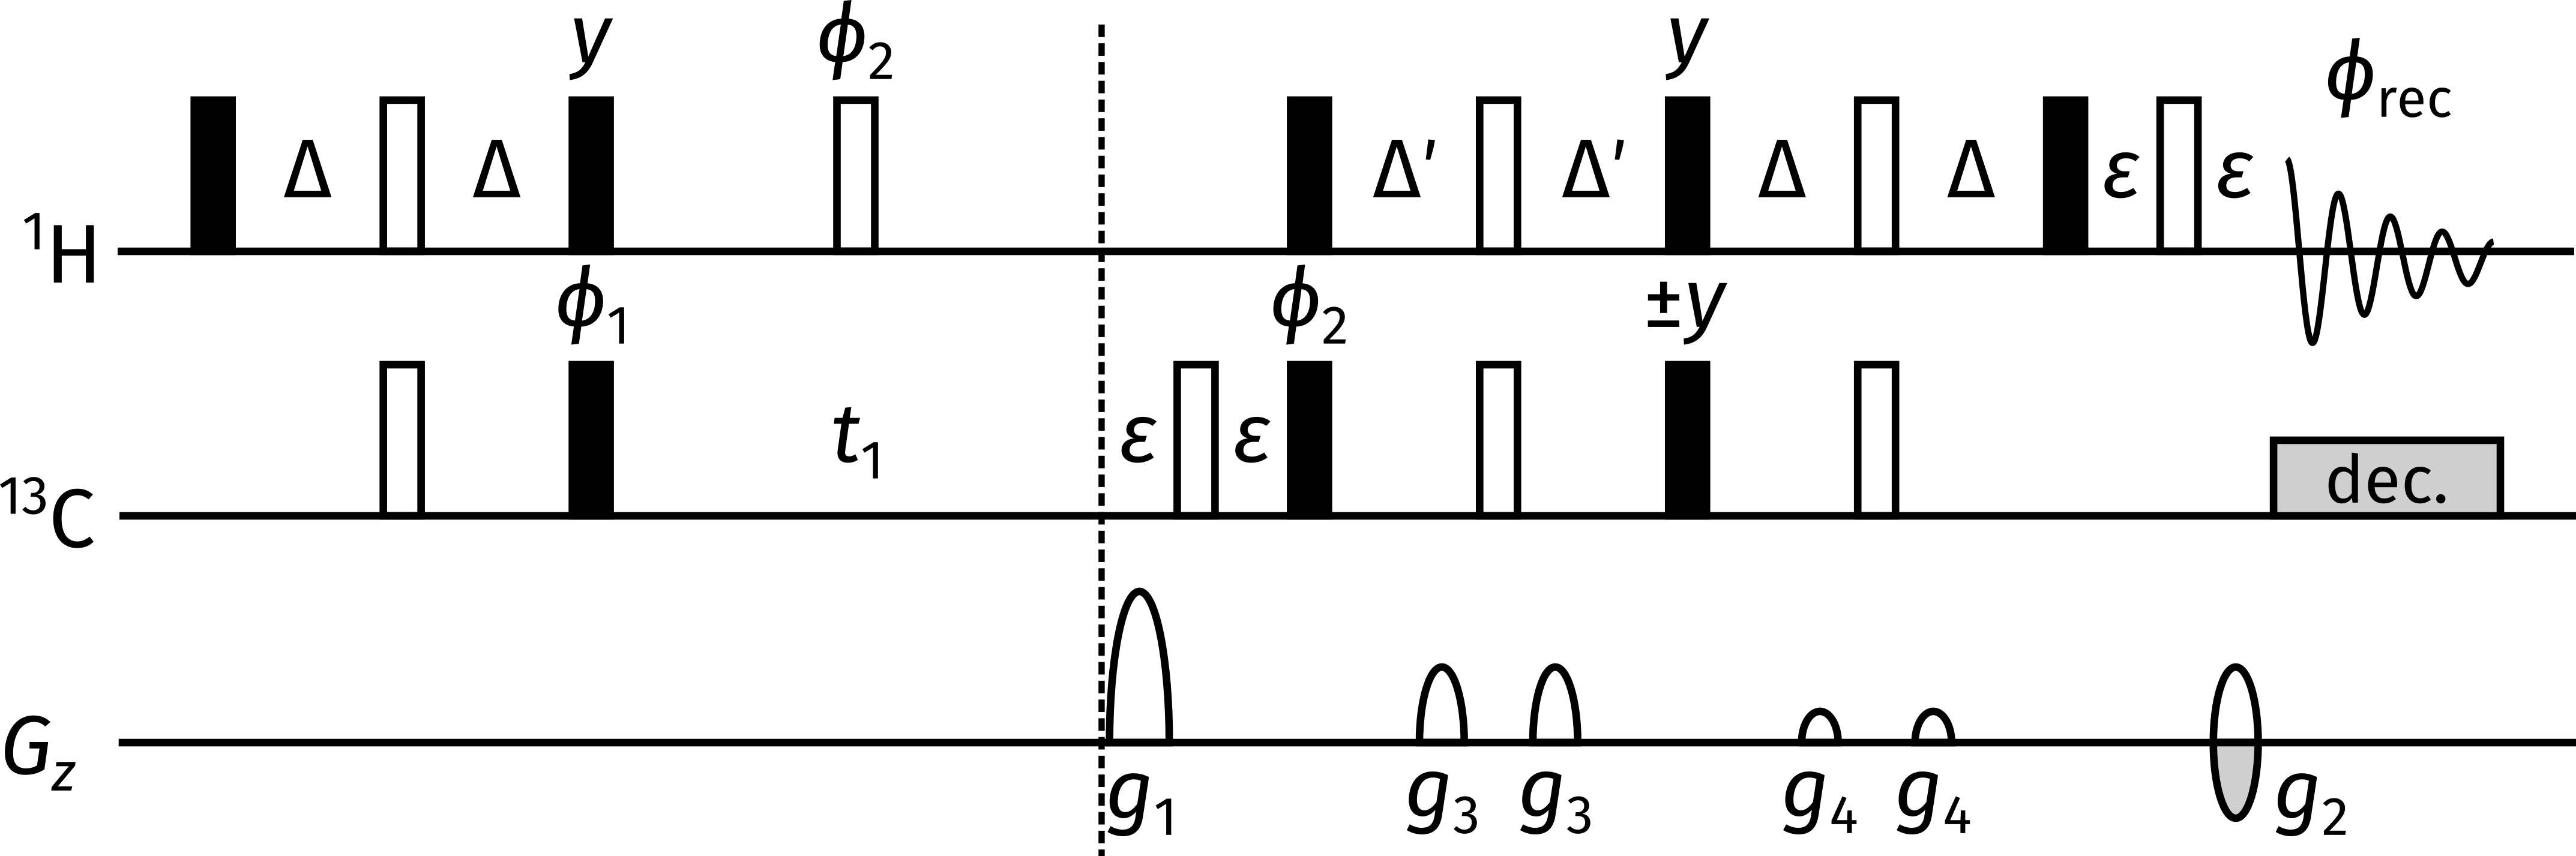
\includegraphics[]{pp/sehsqc/crk_preface.png}
    \caption[Example pulse sequence to illustrate notation]{An example of a pulse sequence (the sensitivity-enhanced HSQC, see \cref{subsec:noah__sehsqc}), used here to illustrate the notation used in this thesis.}
    \label{fig:preface_sehsqc}
\end{figure}

NMR pulse sequences in this thesis are depicted in a reasonably conventional manner: \cref{fig:preface_sehsqc} shows an example of this.
The notation used is described here to avoid any ambiguity.
Filled black rectangular bars indicate \ang{90} pulses; empty bars indicate \ang{180} pulses.
Pulses with other flip angles are depicted using filled grey bars, typically with the Greek letter $\beta$ above it representing the flip angle.
Delays are variously represented by the letters $\Delta$ and $\tau$; exact values of these will be given in the respective captions.
Pulses without explicit phases are assumed to be applied along the rotating-frame $+x$-axis; phases of the form $\phi_i$ are typically cycled during the experiment and will be specified in the captions.
Grey boxes labelled `dec.' represent decoupling periods.

$z$-Gradient amplitudes are given as percentages of the maximum gradient amplitude, which is probe-dependent (see \cref{tbl:spectrometers}).
This maximum amplitude is unlikely to substantially affect the performance of any of the pulse sequences; consequently, in the text I quote gradient amplitudes only as percentages.
Gradients which are inverted for echo--antiecho selection are depicted as a pair of positive and negative gradients (e.g.\ $g_2$ above).
Note that whether the gradient is above or below the $G_z$ line has no direct bearing on the sign of its amplitude (this may, in general, depend on the magnetogyric ratios of the nuclei being detected).
$\varepsilon$ is always used to denote the time required for a pulsed field gradient, plus the subsequent recovery delay.

In practice, the implementation of a pulse sequence may differ in tiny ways: for example delays may be modified to accommodate finite pulse widths and other technicalities.
Furthermore, shaped pulses may be used in place of hard pulses in order to optimise the pulse sequence, e.g.\ by allowing more efficient refocusing or excitation.

\section*{Software}

All NMR data was processed using TopSpin 3 or 4.
Quantum mechanical NMR simulations were done in Matlab R2021a or R2021b.
This thesis is written using the \LaTeX{} typesetting system: specifically, I used the \LuaLaTeX{} engine.

Pulse sequences are drawn using the vector graphics programme \href{https://inkscape.org/}{Inkscape}.
Plots are generated using \href{https://www.python.org/}{Python 3}, using a number of packages (namely: \href{https://github.com/numpy/numpy}{\texttt{numpy}}, \href{https://github.com/scipy/scipy}{\texttt{scipy}}, \href{https://github.com/matplotlib/matplotlib}{\texttt{matplotlib}}, \href{https://github.com/mwaskom/seaborn}{\texttt{seaborn}}, and \href{https://github.com/yongrenjie/penguins}{\texttt{penguins}}, the last of which was written by me, and described further in \cref{sec:other__penguins}).

The underlying \LaTeX{} code for this thesis, as well as all figures, can be accessed at \todo{TODO (likely GitHub)}.

\section*{Samples used}

The caption of every figure showing experimental data includes a `code' at the end, which indicates the spectrometer and sample used for the data, as well as the date (in \texttt{YYMMDD} format).
The available spectrometers and samples are enumerated in \cref{tbl:spectrometers,tbl:samples,fig:samples}.
Therefore, for example, the code \texttt{7Z-211225} would represent data acquired on the \SI{700}{\MHz} spectrometer, using the zolmitriptan sample, on Christmas Day 2021.

\begin{table}
    \begin{tabular}{ccl}
        \toprule
        \textbf{Code} & \textbf{Internal name} & \textbf{Details} \\
        \midrule
        \texttt{7} & \href{http://nmrweb.chem.ox.ac.uk/av700.aspx}{AV700} & \makecell[l]{
             \SI{700}{\MHz} \proton{} resonance frequency \\
             \SI{5}{\mm} TCI \proton{}/\carbon{}/\nitrogen{} inverse cryoprobe \\
             \SI{53}{\gauss\per\cm} maximum $z$-gradient amplitude \\
             AVANCE III console, TopSpin 3.6.2
         } \\
         \midrule
        \texttt{6} & \href{http://nmrweb.chem.ox.ac.uk/av600.aspx}{AV600} & \makecell[l]{
             \SI{600}{\MHz} \proton{} resonance frequency \\
             \SI{5}{\mm} Prodigy \ch{N2} broadband cryoprobe (\proton{}/\fluorine{} outer coil) \\
             \SI{66}{\gauss\per\cm} maximum $z$-gradient amplitude \\
             AVANCE III console, TopSpin 3.6.2
         } \\
        \midrule
        \texttt{5} & \href{http://nmrweb.chem.ox.ac.uk/avx500.aspx}{AVX500} & \makecell[l]{
             \SI{500}{\MHz} \proton{} resonance frequency \\
             \SI{5}{\mm} TBO \proton{}/\fluorine{}/\ch{X} broadband room-temperature  probe \\
             \SI{50}{\gauss\per\cm} maximum $z$-gradient amplitude \\
             AVANCE III console, TopSpin 3.6.2
         } \\
        \midrule
        \texttt{4} & \href{http://nmrweb.chem.ox.ac.uk/avb400.aspx}{AVB400} & \makecell[l]{
             \SI{400}{\MHz} \proton{} resonance frequency \\
             \SI{5}{\mm} broadband (room-temperature) SmartProbe \\
             \SI{50}{\gauss\per\cm} maximum $z$-gradient amplitude \\
             AVANCE NEO console, TopSpin 4.0.8
         } \\
        \bottomrule
    \end{tabular}
    \caption[Spectrometers used in this thesis]{Spectrometers used in this thesis. A more complete description may be accessed via the links in the `internal name' column.}
    \label{tbl:spectrometers}
\end{table}

\begin{table}
    \begin{tabular}{cccc}
        \toprule
        \textbf{Code} & \textbf{Compound} & \textbf{Solvent} & \textbf{Concentration} \\
        \midrule
        \texttt{A}  & Andrographolide & \dmso      & \SI{40}{\milli\molar}  \\
        \texttt{B}  & (3-Fluorophenyl)boronic acid & \dmso & \SI{120}{\milli\molar}  \\
        \texttt{C}  & Cyclosporin A   & \ch{C6D6}  & \SI{50}{\milli\molar}  \\
        \texttt{E}  & Ethanol         & \ch{D2O}   & \SI{1}{\molar}         \\
        \texttt{F}  & Ferulic acid    & \dmso      & \SI{50}{\milli\molar}  \\
        \texttt{G}  & Gramicidin S    & \dmso      & \SI{40}{\milli\molar}  \\
        \texttt{H}  & Cholesterol     & \ch{CDCl3} & \SI{50}{\milli\molar}  \\
        \texttt{S}  & Sucrose         & 90\% \ch{H2O} / 10\% \ch{D2O} & \SI{22}{\milli\molar}  \\
        \texttt{T}  & Ethyl ferulate  & \dmso      & \SI{200}{\milli\molar} \\
        \texttt{X}  & Brucine         & \ch{CDCl3} & \SI{50}{\milli\molar} \\
        \texttt{Z}  & Zolmitriptan    & \dmso      & \SI{50}{\milli\molar}  \\
        \bottomrule
    \end{tabular}
    \caption[Samples used in this thesis]{Samples used in this thesis. Note that concentrations are approximate and not necessarily constant, as samples were remade over time due to e.g.\ decomposition. However, it is reasonable to assume that the variation in concentration is below 10\%. See \cref{fig:samples} for chemical structures.}
    \label{tbl:samples}
\end{table}

\begin{figure}
    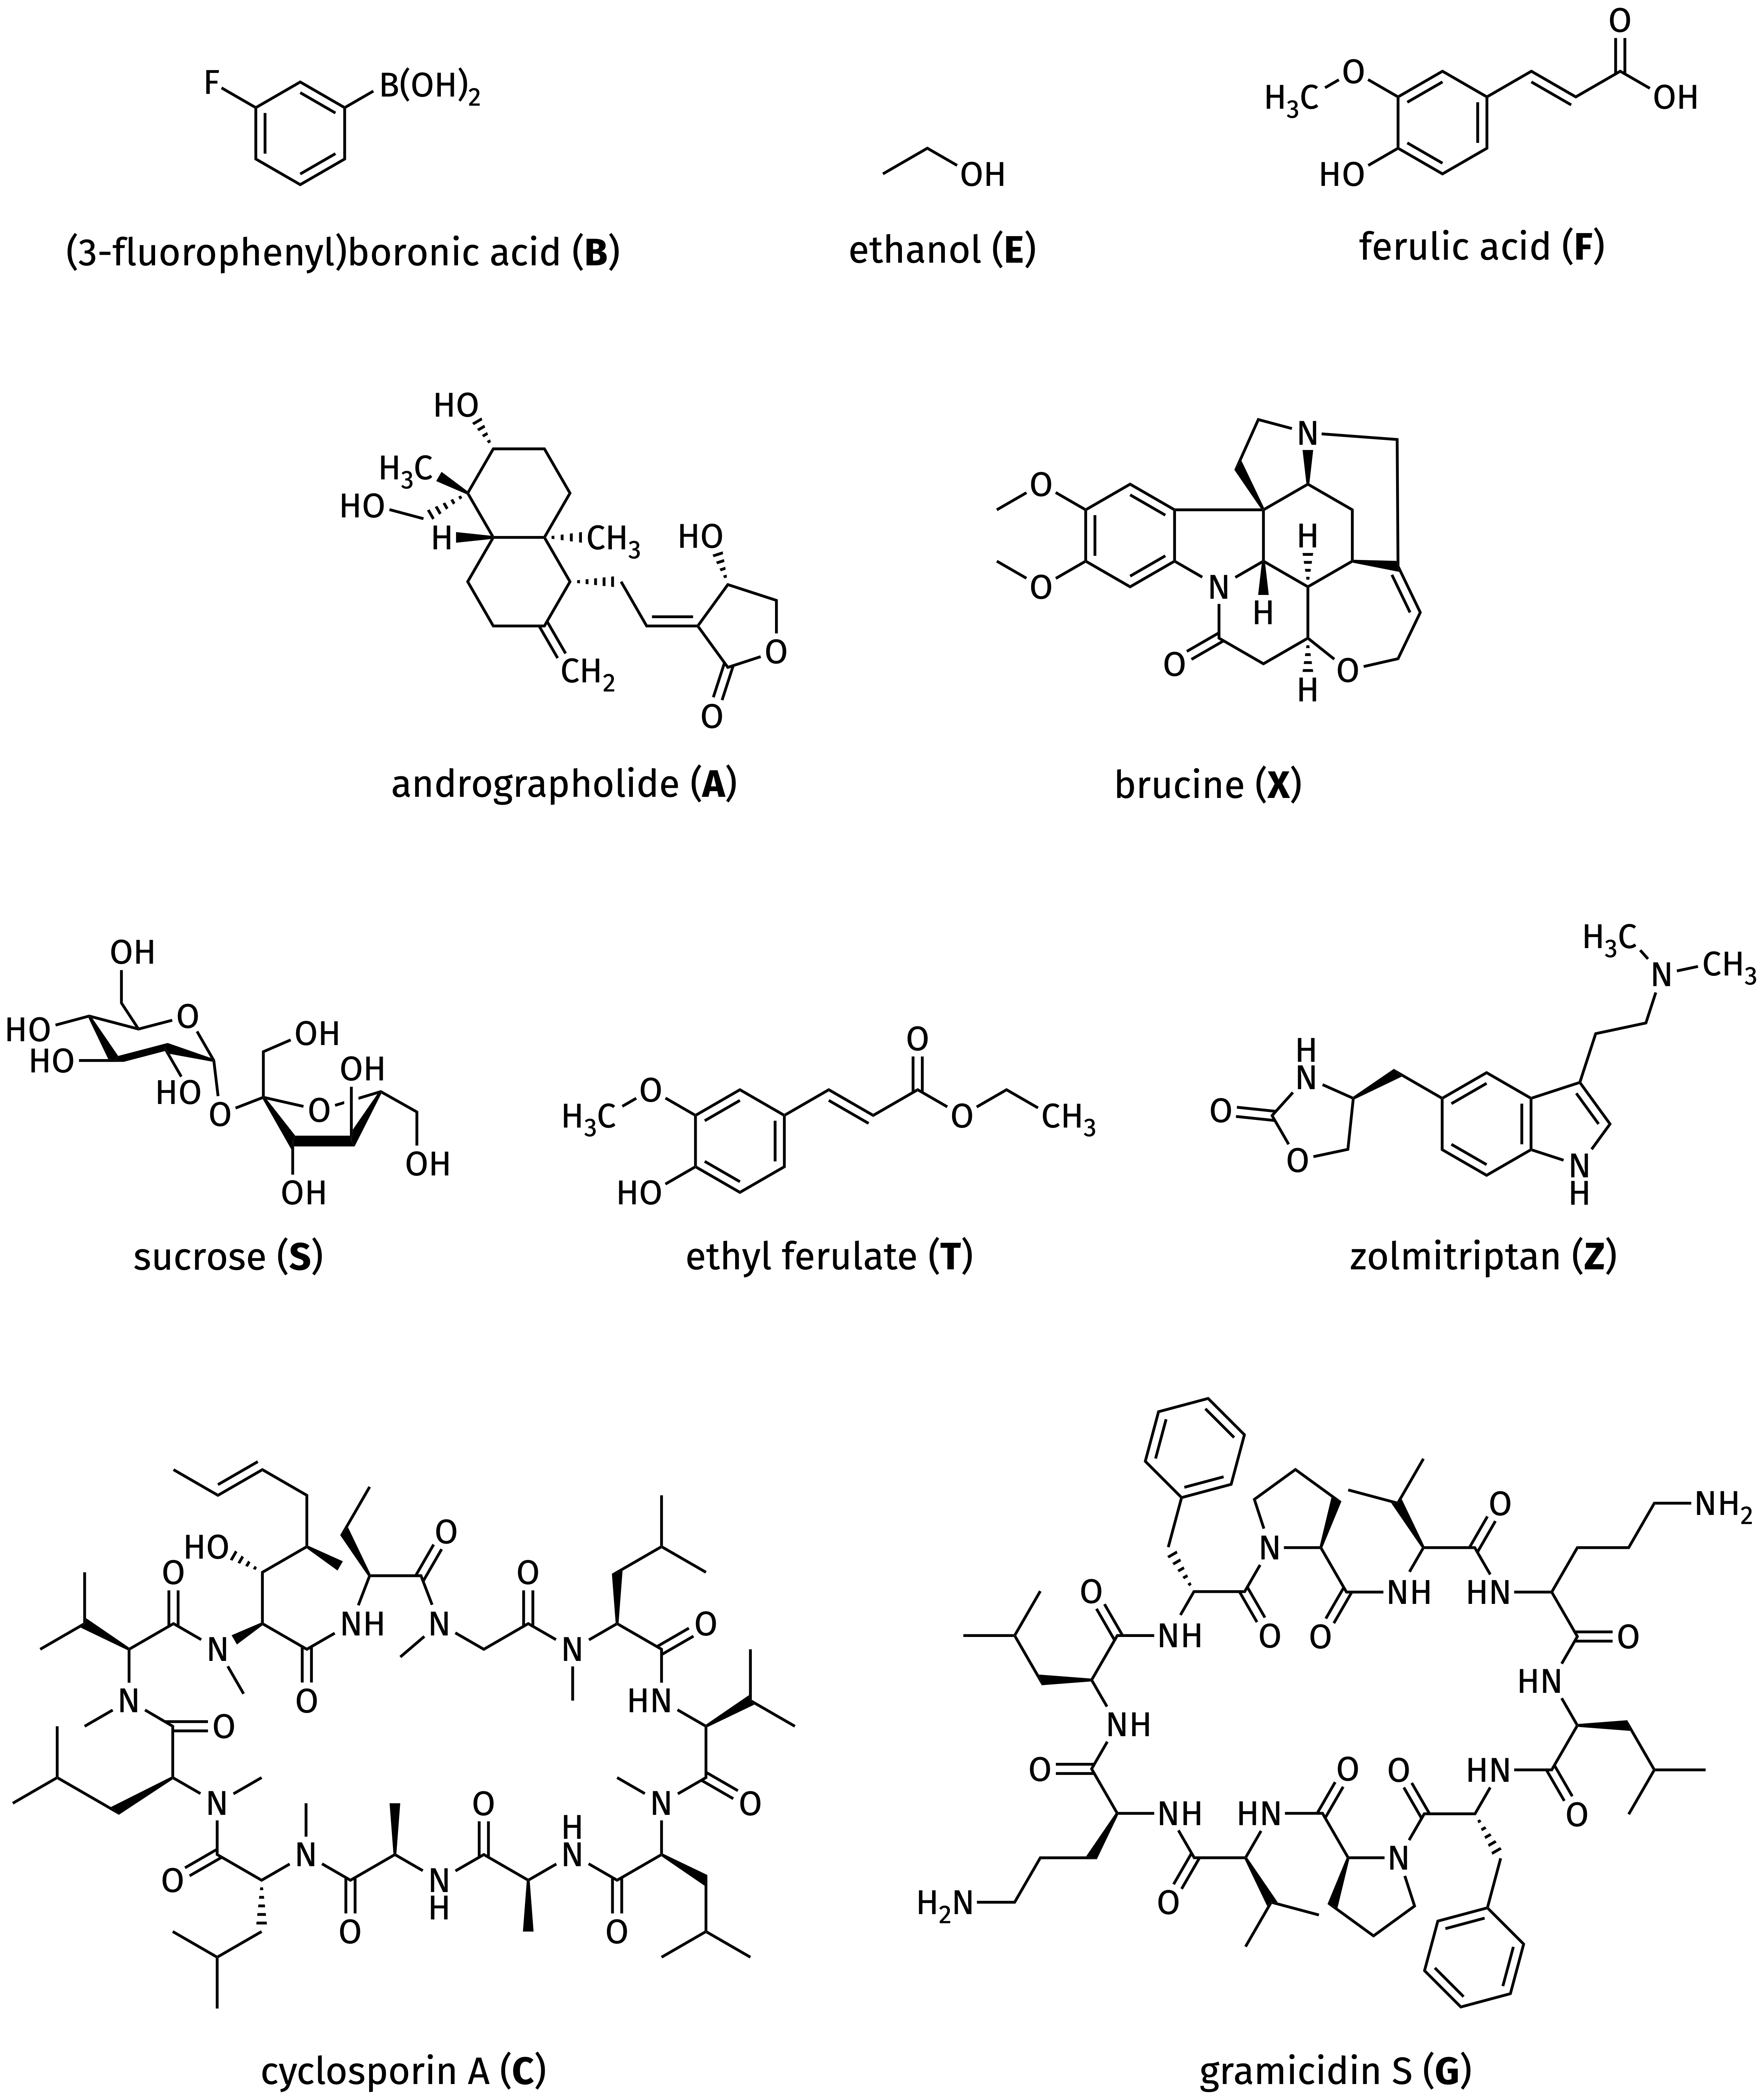
\includegraphics[width=\textwidth]{samples_fira.png}
    \caption[Chemical structures of samples used in this thesis]{Chemical structures of samples used in this thesis. See \cref{tbl:samples} for more information.}
    \label{fig:samples}
\end{figure}
